\documentclass{article}

\usepackage[utf8]{inputenc}
\usepackage{graphicx}
\usepackage[margin=1in]{geometry}
\usepackage{subcaption}

\title{\vspace{30mm}EE382M: VLSI I \\ Monolithic 3D IC Basic Cell Library}

\author {
	Emily~Bragg,~Tengchieh~Huang\\
       	\em emily.bragg@utexas.edu,~tengchieh@utexas.edu\
}

\date{\today}

\begin{document}
\maketitle

\newpage
\section{Introduction}
3D integrated circuits (3DICs) are one potential advancement that will allow circuit designers to save area by having different parts of a design on different layers of silicon which are then bonded together. There are several different styles of 3DIC technology, but we will be focusing on monolithic 3DICs. We designed a standard cell library for 3DIC technology, and simulated the cells to determine the performances differences as compared to the standard version of each cell. 
\section{Technology Background}
\subsection{3D ICs} There are two common types of 3D ICs. The more common variety, which the library we plan to use was designed for, uses Through-Silicon Vias (TSVs) to connect layers, with each layer typically having full transistors. This allows vertical logic, but requires careful planning so as to ensure that the layers line up. Another issue with this approach is that a single TSV is very large relative to the cells it connects; at a 45nm technology node, the minimum width of a TSV is 6000nm ~\cite{NCSU}. This obviously cannot be used for fine-grained modifications to a design, and must be planned for when the design is initially made. 
\subsection{Monolithic 3D ICs} One way of avoiding the problem with TSV is through monolithic 3D IC technology. This technology is also a vertical technology, but it builds up very thin layers of devices instead of bonding them together. Instead of having TSVs, monolithic integration has 'monolithic inter-tier vias' (MIV). These MIVs, at 70nm, are a similar size to the contacts used at a 45nm technology node~\cite{ULTRA}, and thus can be used to design individual cells across multiple layers. They additionally have negligible parasitic capacitance. Because a significant portion of cell area comes from the necessary separation between the pwell and the nwell, by splitting the pull-up network and pull-down networks and putting each on a separate layer, we can achieve significantly smaller area without having to alter logic. We also considered doing the method presented in ~\cite{CELONCEL}; however, due to the limitations of the tools, the advantages of these method (stacking cells on top of other cells by layers to reduce wire lengths and delays across designs) would be difficult to illustrate.

\section{Specifications}
\subsection{Overview} We are designing a library of standard cells (listed in Table \ref{tab:cell_table}) for reducing area using monolithic 3D IC technology. Once completed, these cells should be able to be placed in a design andreduce the area by up to 40\% in the ideal case. This also should allow for less area consumed by routing, as routing can be run in the layer that has less area dedicated to logic (typically the same layer as the NMOS, due to the smaller transistor widths).

\begin{table}[h]
\centering
\begin{tabular}{|c|c|} 
\hline
Cell & Sizes \\ \hline
AND & 2,3,4 \\ \hline
OR & 2,3, 4\\ \hline
NAND & 2, 3,4 \\ \hline
NOR & 2, 3, 4\\ \hline
AOI & 21, 22 \\ \hline
OAI & 21, 22 \\ \hline
INV & N/A \\ \hline
BUF & N/A \\ \hline
\end{tabular}
\caption{Cell Types and Sizes}
\label{tab:cell_table}
\end{table}

\subsection{Interface} The goal of cell design is to ensure that the inputs and outputs match identically with standard cell libraries of traditional technology. As such, each cell has the standard outputs. The primary difference is that the target library has VDD and GND rails stacked on separate layers, and as such they are not at opposing ends of the cell as they traditionally are in standard cells. All inputs and outputs come from the opposite side of the cell from the power and ground rails in our designs. 

\subsection{Design Targets} Our primary goal is area reduction, and we expect that using 3D IC technology can achieve area improvements approaching 50\% in the ideal case. However, we expect most of our better gains to be around 40\% less area, due to the overhead created by the MIVs. The best cases for area reduction come from gates that have equally sized PMOS and NMOS transistors; however, this is rarely the case (with size typically larger on the PMOS network), and even if it were, we could not achieve 50\% area reduction due to the MIV area. We plan to create reference versions of all of the standard cells, and the power and timing requirements for the reference versions are our design targets for the power and timing requirements of the 3D versions. 

\section{Design}
\subsection{Basic Architecture} The most basic goal of our design is to achieve the functionality of each standard cell. 
\subsection{Toolset} NCSU has a library for 3D ICs that we initially considered using. However, while it does support multiple layers, it has no functionality for MIVs (focusing rather on TSV-based ICs). This meant two things for our design. Firstly, if we built our designs using the 3D IC library provided, there would be no way of achieving power and timing simulation, as TSV technology has radically different effects. Secondly, TSVs would dominate the area of any cell, and thus we would not be able to get valid area results either. The only advantage this path would have had would be for purposes of simulating the logic, which was basic and thus would not be important information. \\ 
We instead decided to utilize the standard 45nm NCSU libraries. While this does not support laying directly, we were able to simulate the effect of the MIV by separating the layers with a metal1 wire, with the length calculate to provide the same resistance as the MIV would, for power and timing simulations. Additionally, as the contacts connecting the poly to the wire are within 5nm of the size of a MIV, we can accurately measure the area. This approach allowed us to calculate the area, power, and timing achievable if we had tools that supported the technology. 
\subsection{Optimization Techniques} We employed the standard optimization techniques used for standard cell libraries, as the pull-up and pull-down networks remain intact. These include sizing the transistors so that they are balanced, adding additional pins on the larger transistors to reduce the resistance from the contacts, and carefully routing the metal1 so as to avoid unnecessary area due to routing. The last one is particularly relevant, as space that would have been available between transistors due to minimum distances between wells is no longer available. One unique advantage that monolithic 3D IC technology gives us is the ability to reduce the length of the poly. As it notes in ~\cite{ULTRA}, the unit resistance of polysilicon is significantly higher than that of metal; by only having polysilicon on the transistor and not forming a wire between them, we can reduce the internal wire resistance. This counteracts the additional resistance provided by the MIV, producing what we anticipate to be a negligible timing difference.  
\subsection{Naming Conventions} Our naming conventions were to have either \textless CELLNAME\textgreater \textless CELLSIZE\textgreater, for a standard version of a cell, or \textless CELLNAME\textgreater \textless CELLSIZE\textgreater\_3D, for the version that has the additional wiring to simulate a 3D IC. 
\subsection{Issue Tracking} We kept track of the cells through git, using it to track progress, bugs, to-do items, and notes on each design as we worked on them. 


\section{User Document}
%data sheet and tables
% need timing, power, area, capacitance, drive strength

\section{Testing}
%testing methods, bugs encountered, traces applied

\section{Optimization}
\subsection{Optimizing Individual Cells}
\subsection{Using Monolithic 3D ICs to Optimize Full Designs}

\paragraph{}


\newpage
\appendix 
\section{Source Code}

\section{Cell Layouts} 

\begin{figure}[h]
\centering
\parbox{8cm}{
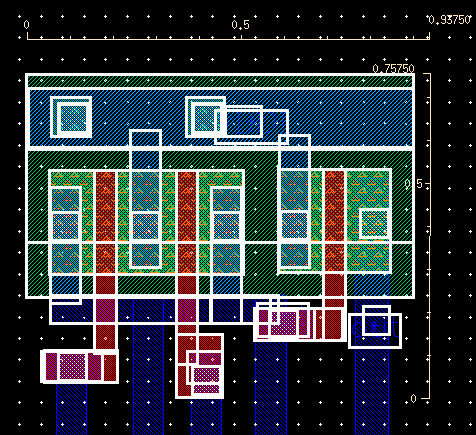
\includegraphics[width=7cm]{final_cells/AND2_PMOS}
  \caption{AND2 Pull-up Network}
\label{fig:AND2_pmos}}
\qquad
\begin{minipage}{7cm}
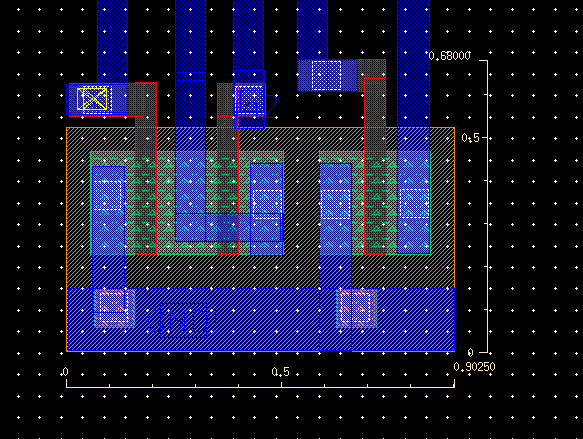
\includegraphics[width=7cm]{final_cells/AND2_NMOS}
  \caption{AND2 Pull-down Network}
\label{fig:AND2_nmos}
\end{minipage}
\end{figure}

\begin{figure}[h]
\centering
\parbox{8cm}{
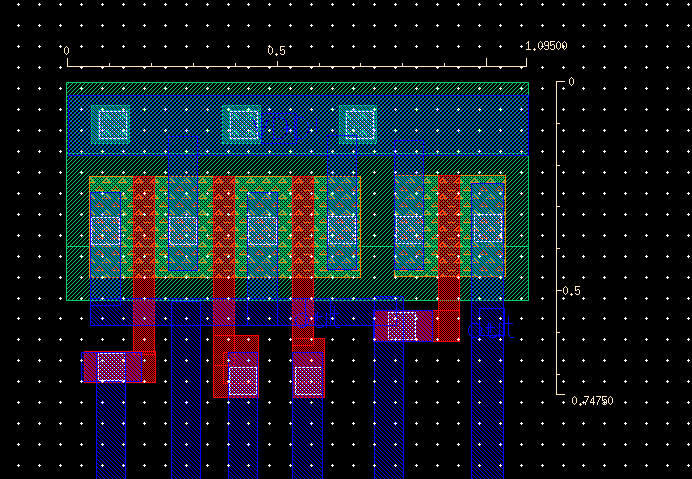
\includegraphics[width=7cm]{final_cells/AND3_PMOS}
  \caption{AND3 Pull-up Network}
\label{fig:AND3_pmos}}
\qquad
\begin{minipage}{7cm}
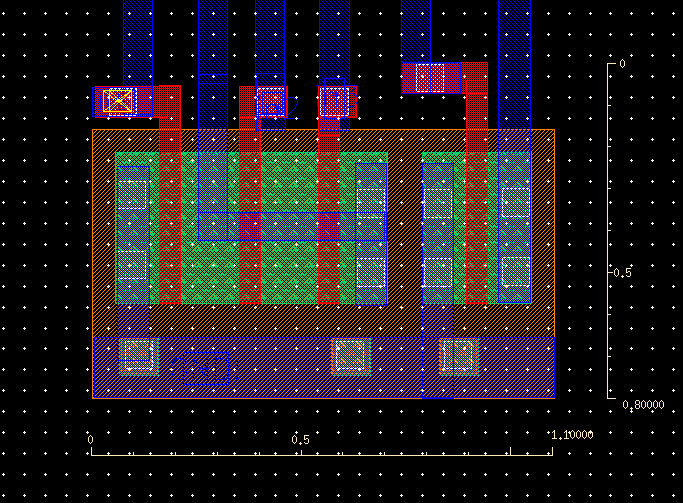
\includegraphics[width=7cm]{final_cells/AND3_NMOS}
  \caption{AND3 Pull-down Network}
\label{fig:AND3_nmos}
\end{minipage}
\end{figure}


\begin{figure}[h]
\centering
\parbox{8cm}{
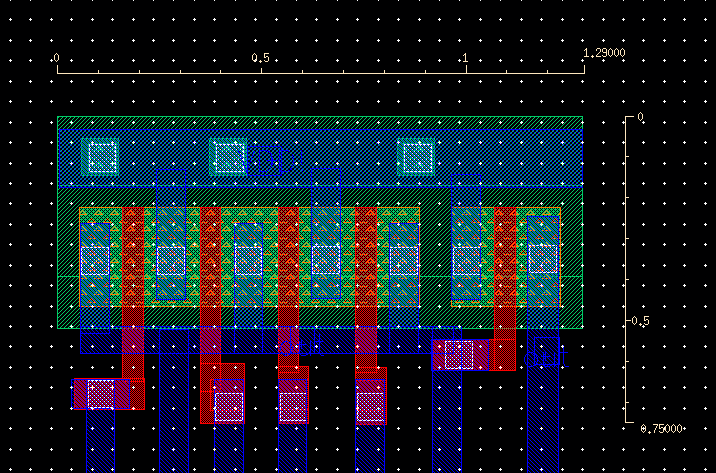
\includegraphics[width=7cm]{final_cells/AND4_PMOS}
  \caption{AND4 Pull-up Network}
\label{fig:AND4_pmos}}
\qquad
\begin{minipage}{7cm}
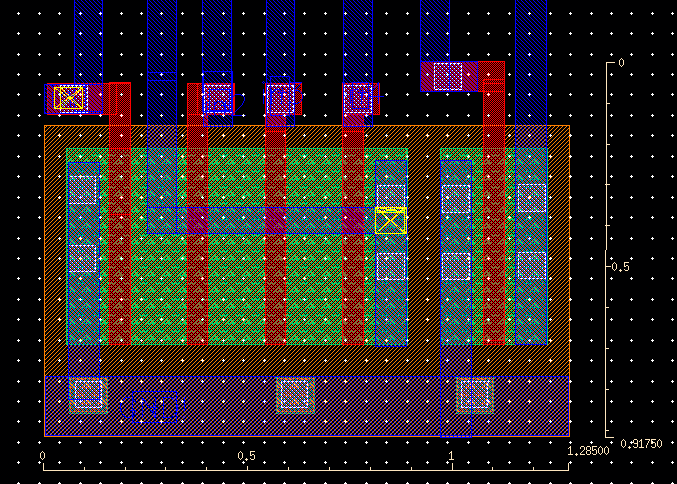
\includegraphics[width=7cm]{final_cells/AND4_NMOS}
  \caption{AND4 Pull-down Network}
\label{fig:AND4_nmos}
\end{minipage}
\end{figure}

\begin{figure}[h]
\centering
\parbox{8cm}{
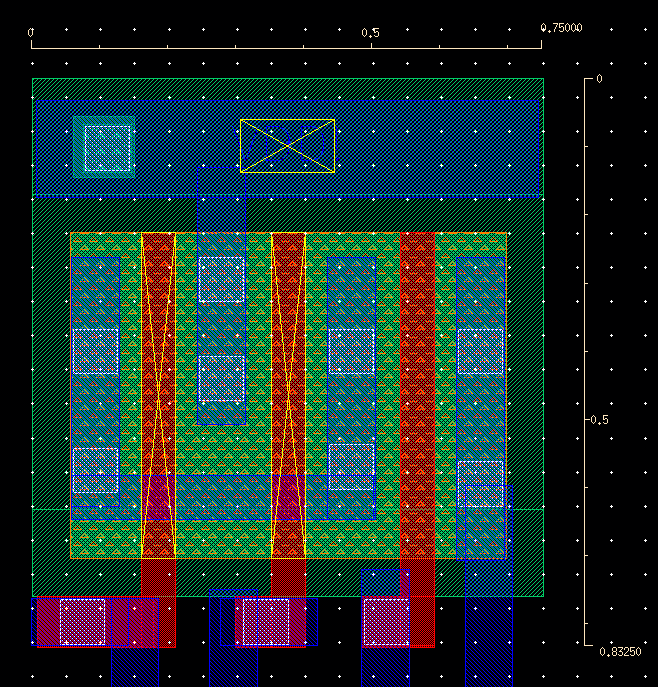
\includegraphics[width=7cm]{final_cells/AOI21_PMOS}
  \caption{AOI21 Pull-up Network}
\label{fig:AOI21_pmos}}
\qquad
\begin{minipage}{7cm}
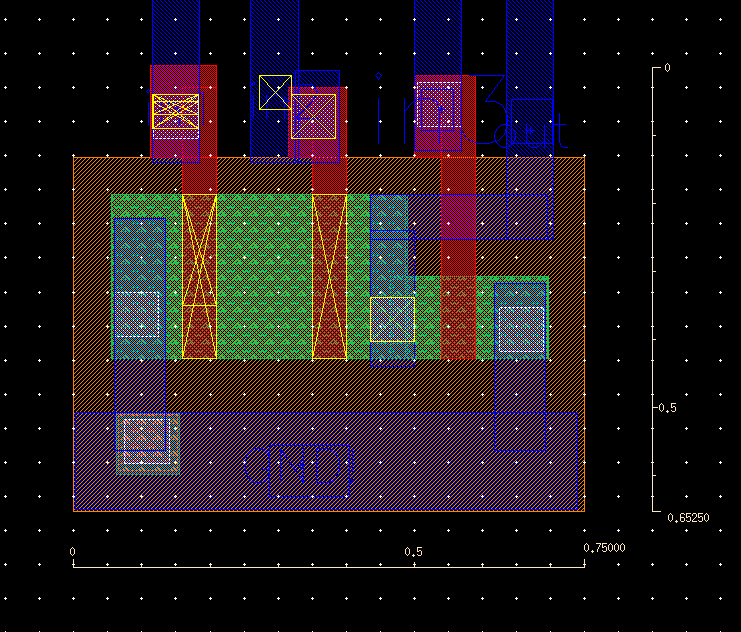
\includegraphics[width=7cm]{final_cells/AOI21_NMOS}
  \caption{AOI21 Pull-down Network}
\label{fig:AOI21_nmos}
\end{minipage}
\end{figure}

\begin{figure}[h]
\centering
\parbox{8cm}{
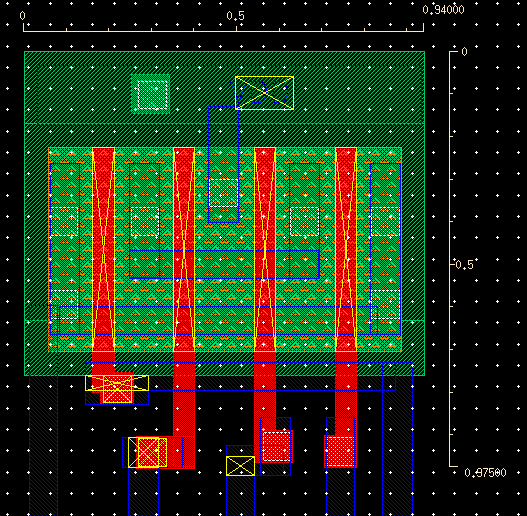
\includegraphics[width=7cm]{final_cells/AOI22_PMOS}
  \caption{AOI22 Pull-up Network}
\label{fig:AOI22_pmos}}
\qquad
\begin{minipage}{7cm}
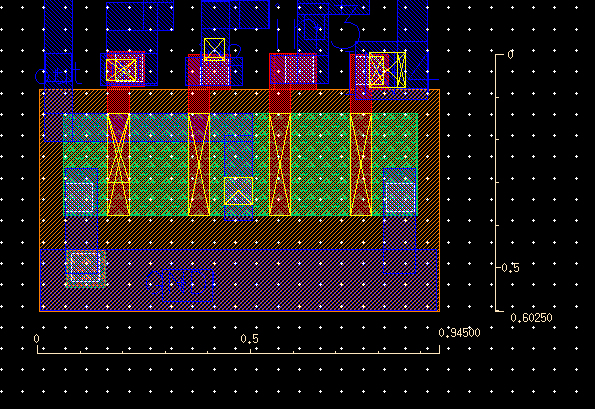
\includegraphics[width=7cm]{final_cells/AOI22_NMOS}
  \caption{AOI22 Pull-down Network}
\label{fig:AOI22_nmos}
\end{minipage}
\end{figure}

\begin{figure}[h]
\centering
\parbox{8cm}{
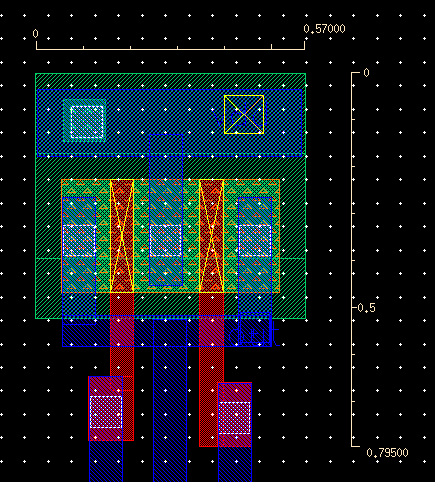
\includegraphics[width=7cm]{final_cells/NAND2_PMOS}
  \caption{NAND2 Pull-up Network}
\label{fig:NAND2_pmos}}
\qquad
\begin{minipage}{7cm}
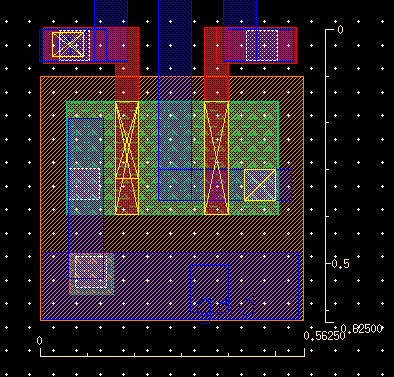
\includegraphics[width=7cm]{final_cells/NAND2_NMOS}
  \caption{NAND2 Pull-down Network}
\label{fig:NAND2_nmos}
\end{minipage}
\end{figure}

\begin{figure}[h]
\centering
\parbox{8cm}{
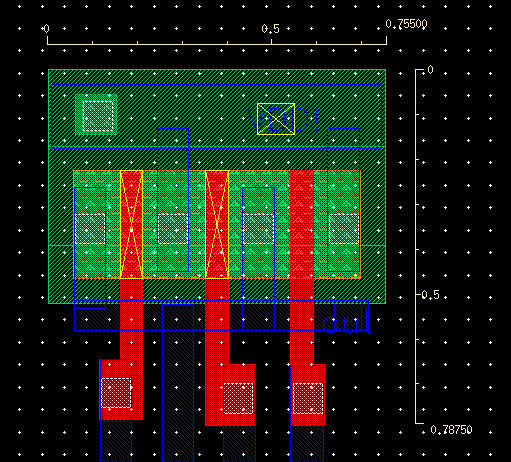
\includegraphics[width=7cm]{final_cells/NAND3_PMOS}
  \caption{NAND3 Pull-up Network}
\label{fig:NAND3_pmos}}
\qquad
\begin{minipage}{7cm}
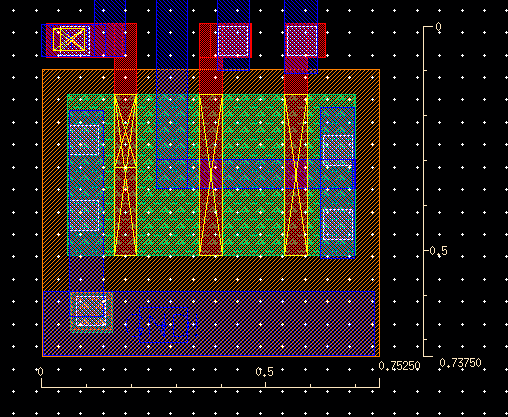
\includegraphics[width=7cm]{final_cells/NAND3_NMOS}
  \caption{NAND3 Pull-down Network}
\label{fig:NAND3_nmos}
\end{minipage}
\end{figure}

\begin{figure}[h]
\centering
\parbox{8cm}{
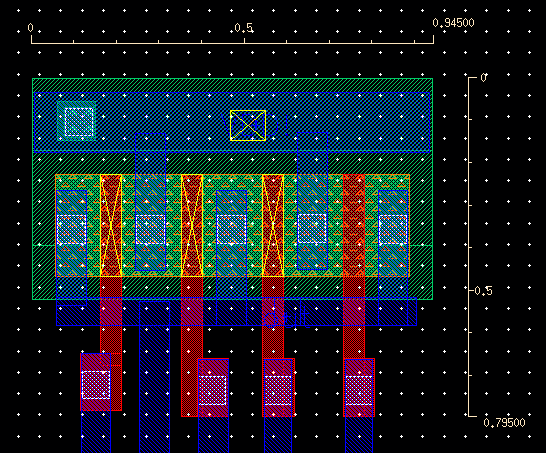
\includegraphics[width=7cm]{final_cells/NAND4_PMOS}
  \caption{NAND4 Pull-up Network}
\label{fig:NAND4_pmos}}
\qquad
\begin{minipage}{7cm}
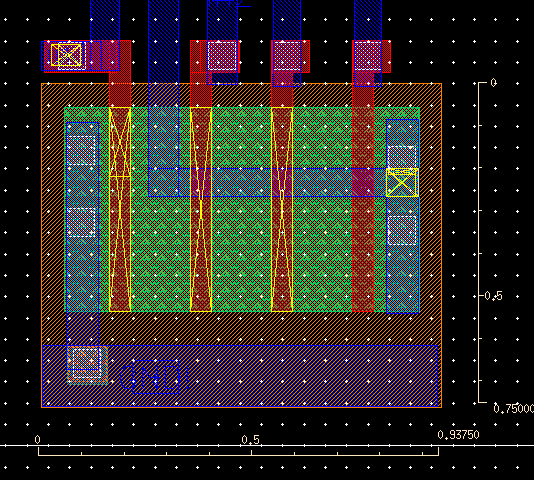
\includegraphics[width=7cm]{final_cells/NAND4_NMOS}
  \caption{NAND4 Pull-down Network}
\label{fig:NAND4_nmos}
\end{minipage}
\end{figure}

\begin{figure}[h]
\centering
\parbox{8cm}{
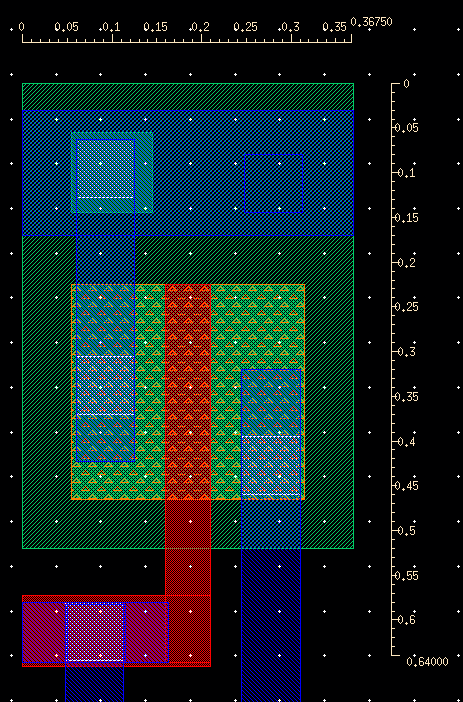
\includegraphics[width=7cm]{final_cells/INV_PMOS}
  \caption{INV Pull-up Network}
\label{fig:INV_pmos}}
\qquad
\begin{minipage}{7cm}
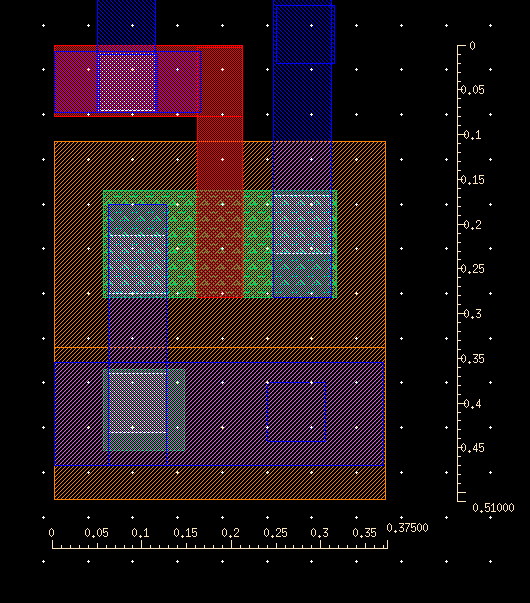
\includegraphics[width=7cm]{final_cells/INV_NMOS}
  \caption{INV Pull-down Network}
\label{fig:INV_nmos}
\end{minipage}
\end{figure}

\begin{figure}[h]
\centering
\parbox{8cm}{
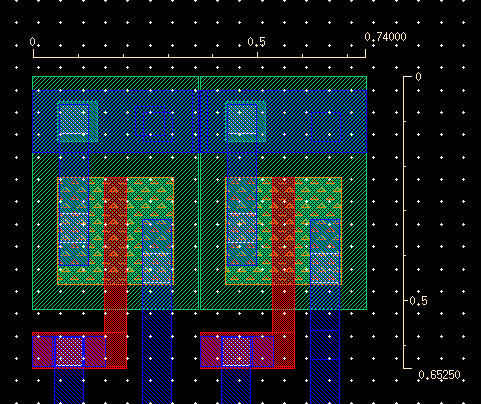
\includegraphics[width=7cm]{final_cells/BUF_PMOS}
  \caption{BUF Pull-up Network}
\label{fig:BUF_pmos}}
\qquad
\begin{minipage}{7cm}
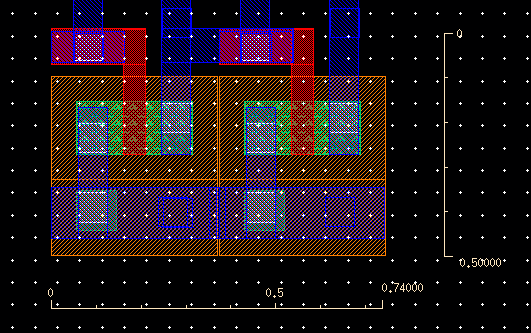
\includegraphics[width=7cm]{final_cells/BUF_NMOS}
  \caption{BUF Pull-down Network}
\label{fig:BUF_nmos}
\end{minipage}
\end{figure}

\begin{figure}[h]
\centering
\parbox{8cm}{
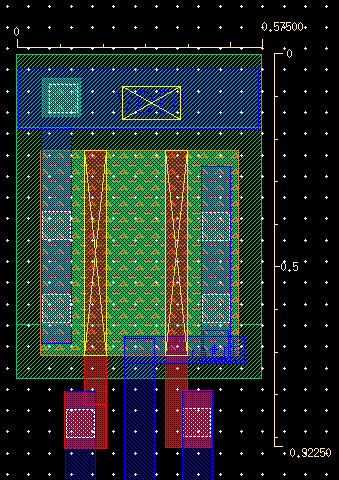
\includegraphics[width=7cm]{final_cells/NOR2_PMOS}
  \caption{NOR2 Pull-up Network}
\label{fig:NOR2_pmos}}
\qquad
\begin{minipage}{7cm}
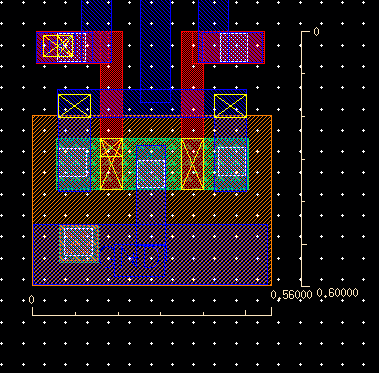
\includegraphics[width=7cm]{final_cells/NOR2_NMOS}
  \caption{NOR2 Pull-down Network}
\label{fig:NOR2_nmos}
\end{minipage}
\end{figure}

\begin{figure}[h]
\centering
\parbox{8cm}{
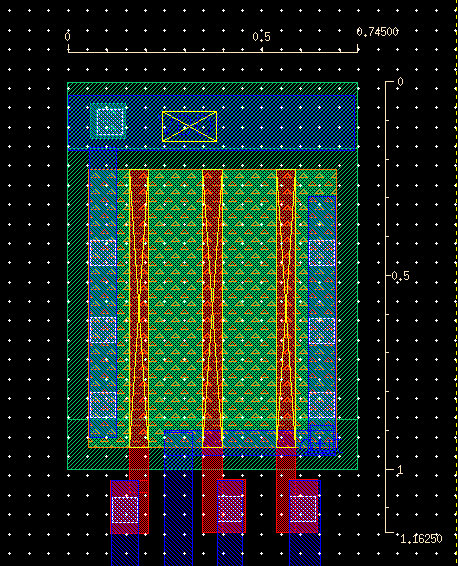
\includegraphics[width=7cm]{final_cells/NOR3_PMOS}
  \caption{NOR3 Pull-up Network}
\label{fig:NOR3_pmos}}
\qquad
\begin{minipage}{7cm}
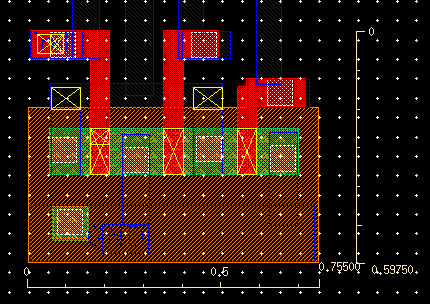
\includegraphics[width=7cm]{final_cells/NOR3_NMOS}
  \caption{NOR3 Pull-down Network}
\label{fig:NOR3_nmos}
\end{minipage}
\end{figure}

\begin{figure}[h]
\centering
\parbox{8cm}{
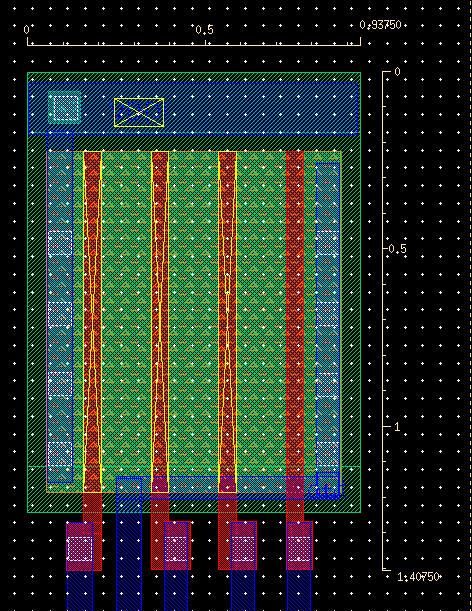
\includegraphics[width=7cm]{final_cells/NOR4_PMOS}
  \caption{NOR4 Pull-up Network}
\label{fig:NOR4_pmos}}
\qquad
\begin{minipage}{7cm}
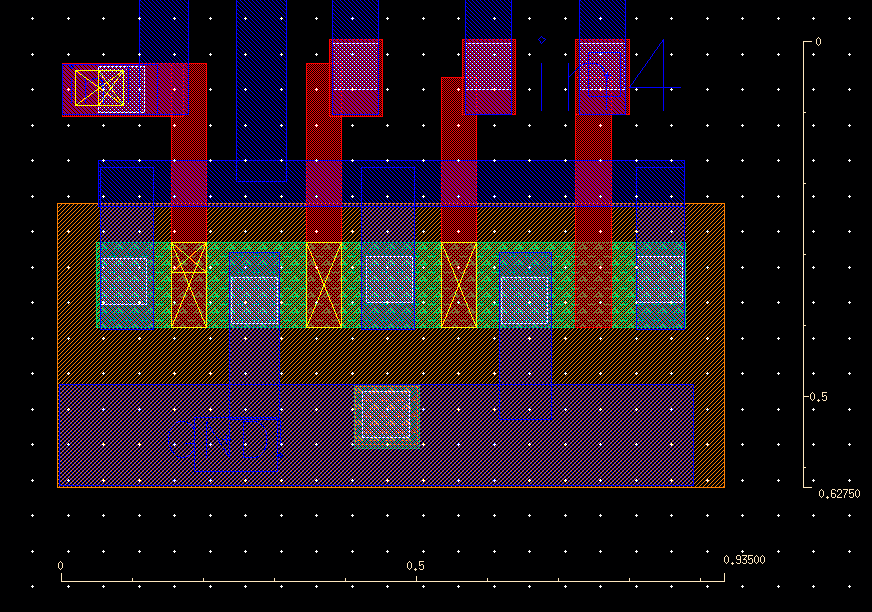
\includegraphics[width=7cm]{final_cells/NOR4_NMOS}
  \caption{NOR4 Pull-down Network}
\label{fig:NOR4_nmos}
\end{minipage}
\end{figure}

\begin{figure}[h]
\centering
\parbox{8cm}{
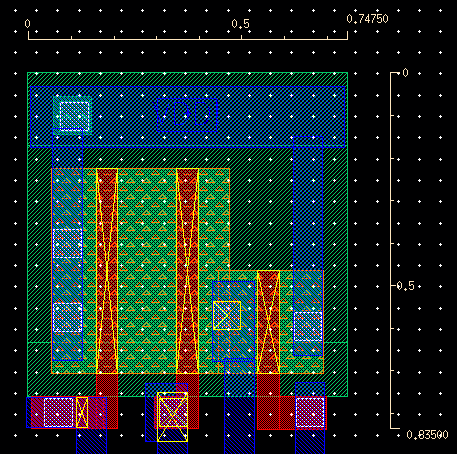
\includegraphics[width=7cm]{final_cells/OAI21_PMOS}
  \caption{OAI21 Pull-up Network}
\label{fig:OAI21_pmos}}
\qquad
\begin{minipage}{7cm}
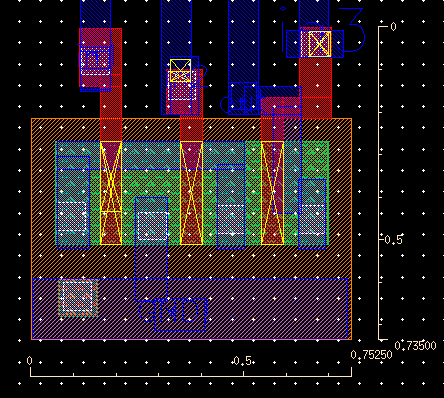
\includegraphics[width=7cm]{final_cells/OAI21_NMOS}
  \caption{OAI21 Pull-down Network}
\label{fig:OAI21_nmos}
\end{minipage}
\end{figure}

\begin{figure}[h]
\centering
\parbox{8cm}{
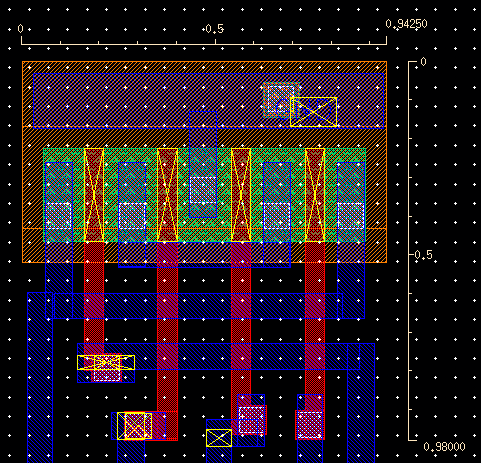
\includegraphics[width=7cm]{final_cells/OAI22_PMOS}
  \caption{OAI22 Pull-up Network}
\label{fig:OAI22_pmos}}
\qquad
\begin{minipage}{7cm}
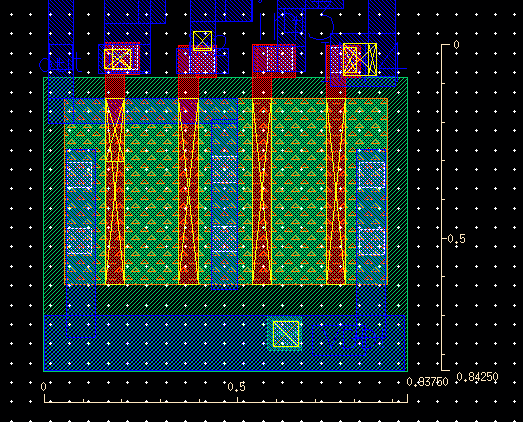
\includegraphics[width=7cm]{final_cells/OAI22_NMOS}
  \caption{OAI22 Pull-down Network}
\label{fig:OAI22_nmos}
\end{minipage}
\end{figure}

\begin{figure}[h]
\centering
\parbox{8cm}{
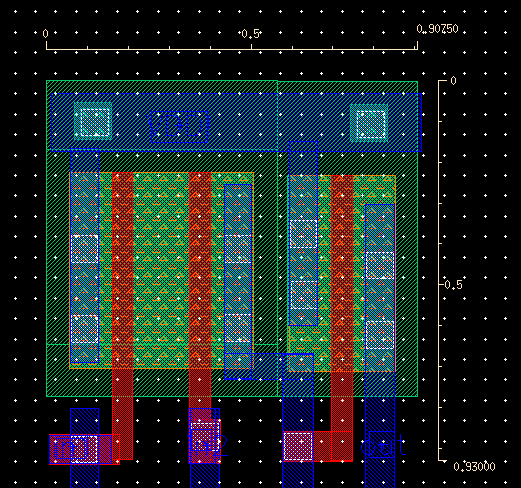
\includegraphics[width=7cm]{final_cells/OR2_PMOS}
  \caption{OR2 Pull-up Network}
\label{fig:OR2_pmos}}
\qquad
\begin{minipage}{7cm}
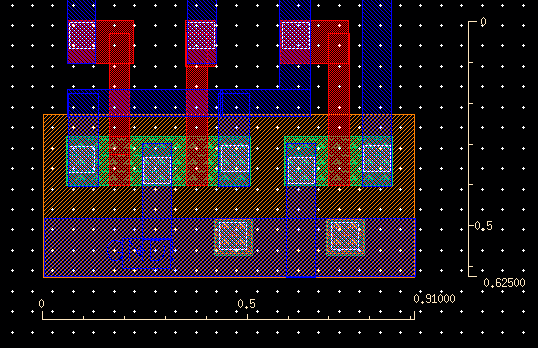
\includegraphics[width=7cm]{final_cells/OR2_NMOS}
  \caption{OR2 Pull-down Network}
\label{fig:OR2_nmos}
\end{minipage}
\end{figure}

\begin{figure}[h]
\centering
\parbox{8cm}{
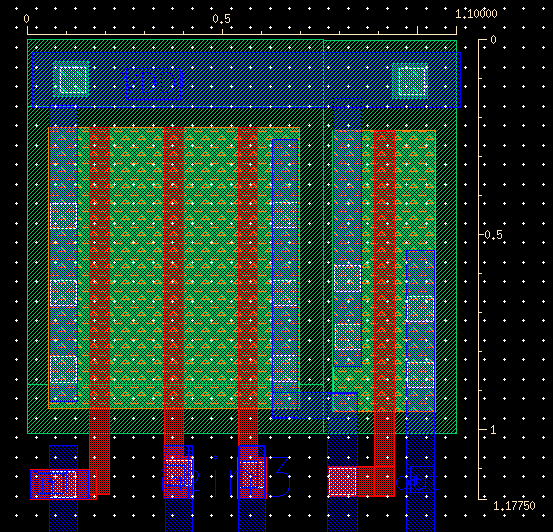
\includegraphics[width=7cm]{final_cells/OR3_PMOS}
  \caption{OR3 Pull-up Network}
\label{fig:OR3_pmos}}
\qquad
\begin{minipage}{7cm}
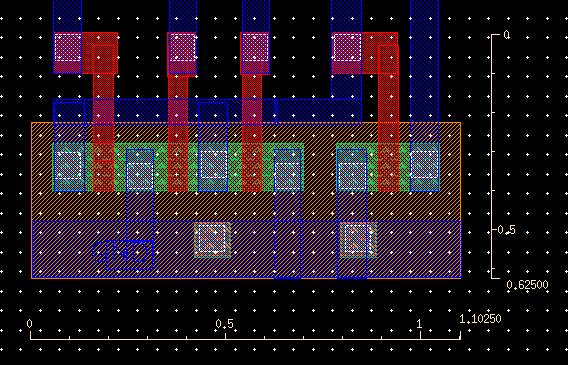
\includegraphics[width=7cm]{final_cells/OR3_NMOS}
  \caption{OR3 Pull-down Network}
\label{fig:OR3_nmos}
\end{minipage}
\end{figure}

\begin{figure}[h]
\centering
\parbox{8cm}{
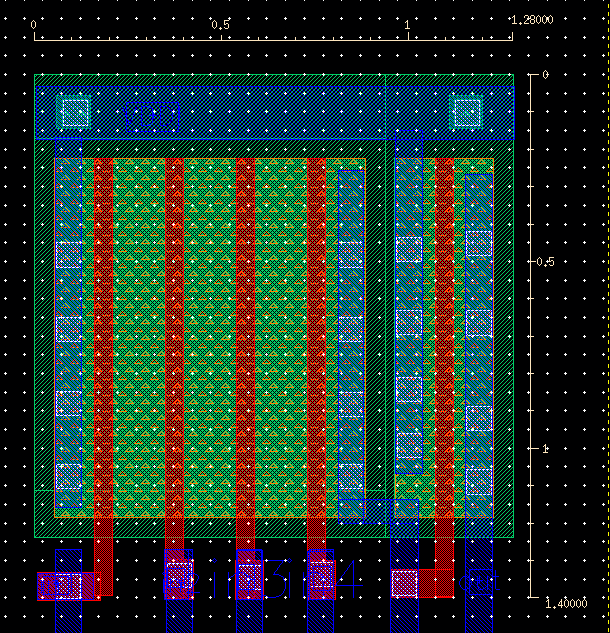
\includegraphics[width=7cm]{final_cells/OR4_PMOS}
  \caption{OR4 Pull-up Network}
\label{fig:OR4_pmos}}
\qquad
\begin{minipage}{7cm}
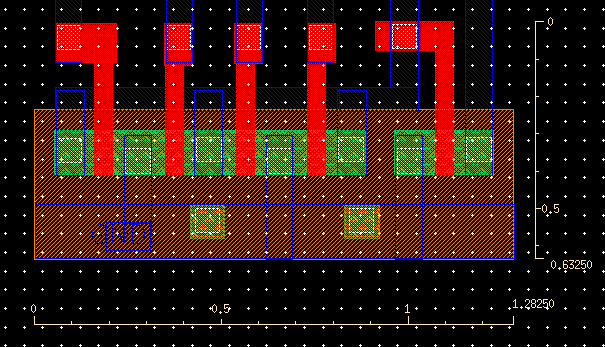
\includegraphics[width=7cm]{final_cells/OR4_NMOS}
  \caption{OR4 Pull-down Network}
\label{fig:OR4_nmos}
\end{minipage}
\end{figure}


\newpage
\bibliographystyle{plain}
\bibliography{vlsi}
\newpage
\end{document}
